\documentclass{beamer} %If no option is specified, 10pt is assumed

\usepackage[sc]{mathpazo} % Use the Palatino font
\usepackage[T1]{fontenc} % Use 8-bit encoding that has 256 glyphs
\linespread{1.05} % Line spacing - Palatino needs more space between lines
\usepackage{microtype} % Slightly tweak font spacing for aesthetics
\usepackage{csquotes}
\usepackage[english]{babel} % Language hyphenation and typographical rules
\usepackage{graphicx}
\usepackage{float}
\usepackage{wrapfig}
\usepackage{circuitikz}
\usepackage{amsmath,amssymb}
\usepackage{geometry} % Document margins, margin=0.6in wasn't there first.
\usepackage[hang, small,labelfont=bf,up,textfont=it,up]{caption} % Custom captions under/above floats in tables or figures
\usepackage{booktabs} % Horizontal rules in tables

\usepackage{lettrine} % The lettrine is the first enlarged letter at the beginning of the text

\usepackage{enumitem} % Customized lists
\setlist[itemize]{noitemsep} % Make itemize lists more compact

\setlength{\headheight}{13.59999pt} % make fancyheader stop complaining

%----------------------------------------------------------------------------------------
%	TITLE SECTION
%----------------------------------------------------------------------------------------

\title{RFEA scan results} % Article title
\author{Arthur Adriaens}
\date{2025}

\begin{document}

% Print the title
\frame{\titlepage}

\begin{frame}
    \frametitle{semion result}
    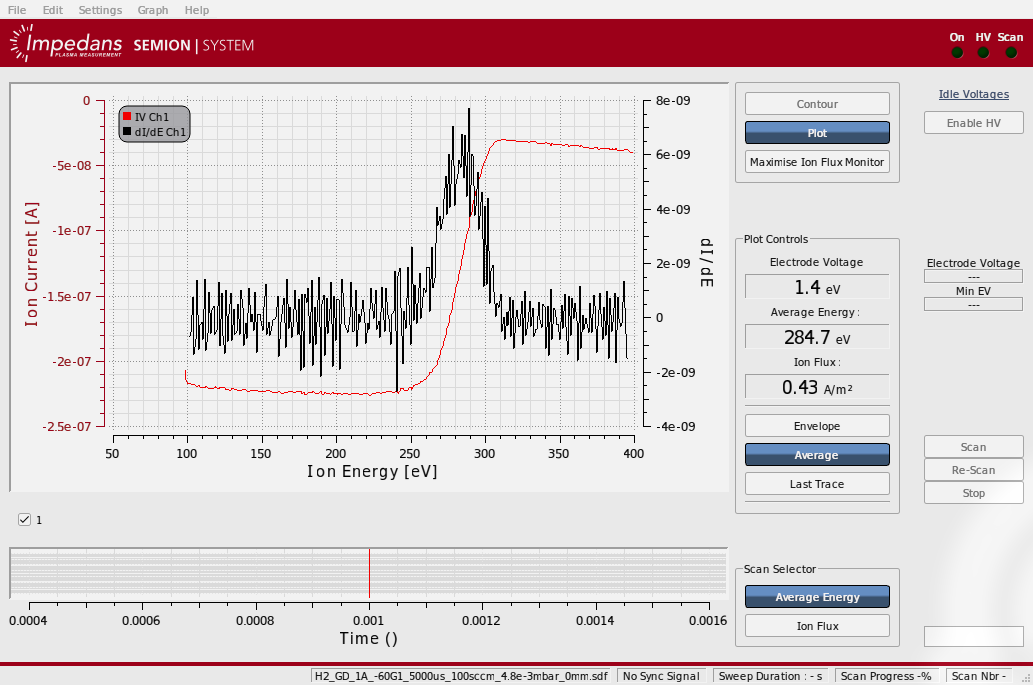
\includegraphics[width=\textwidth]{figures/semion.png}
\end{frame}
\begin{frame}
    \frametitle{multiple traces $\rightarrow$ errors}
    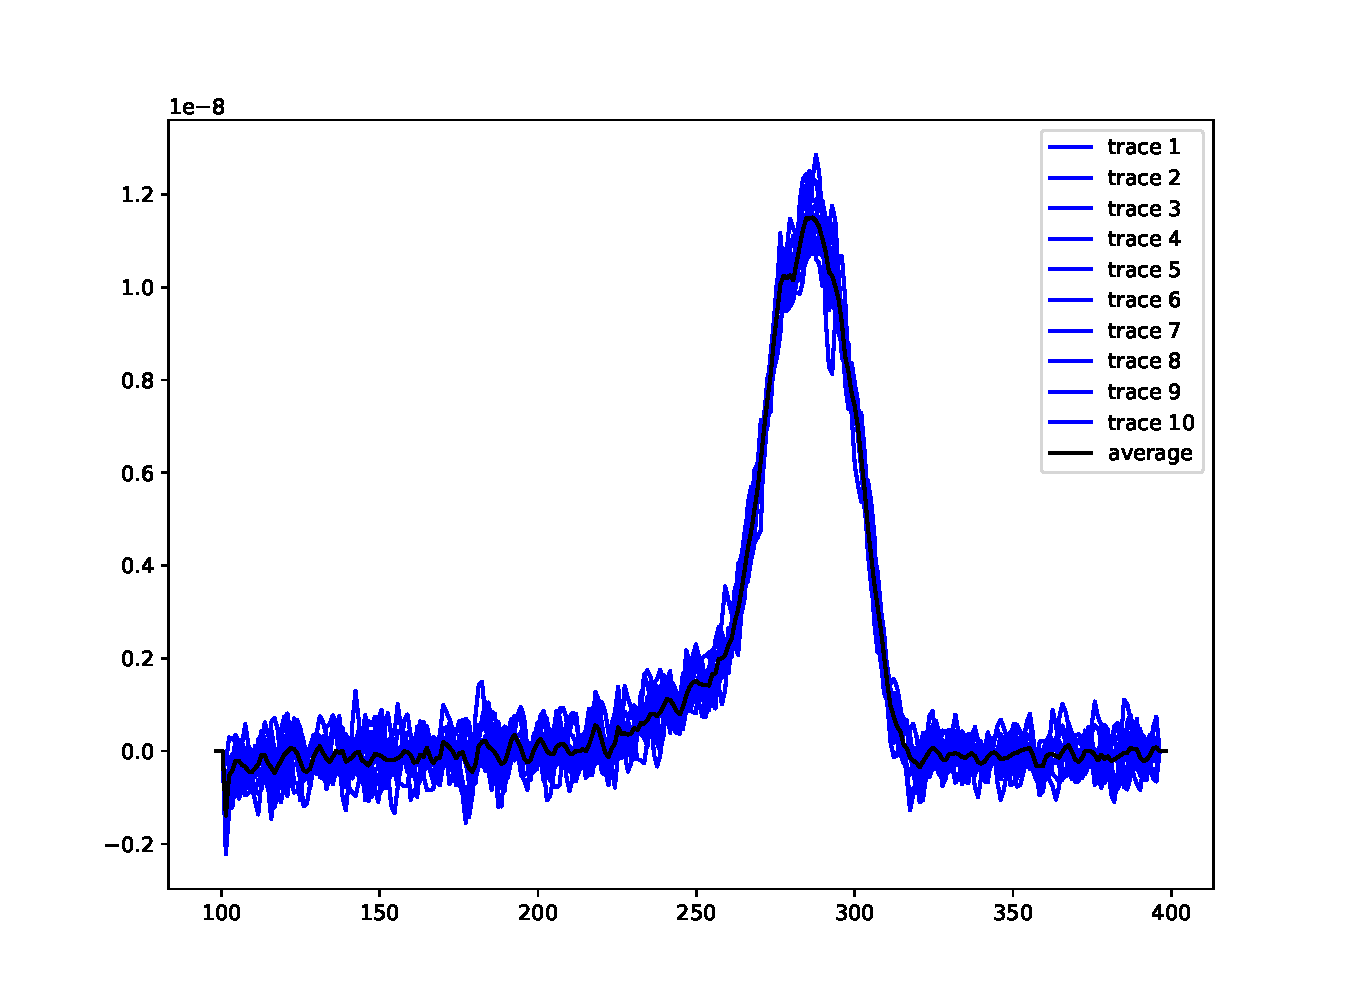
\includegraphics[width=\textwidth]{figures/traces.pdf}
\end{frame}
\begin{frame}
    \frametitle{simple transform to usable distribution (flux vs energy)}
    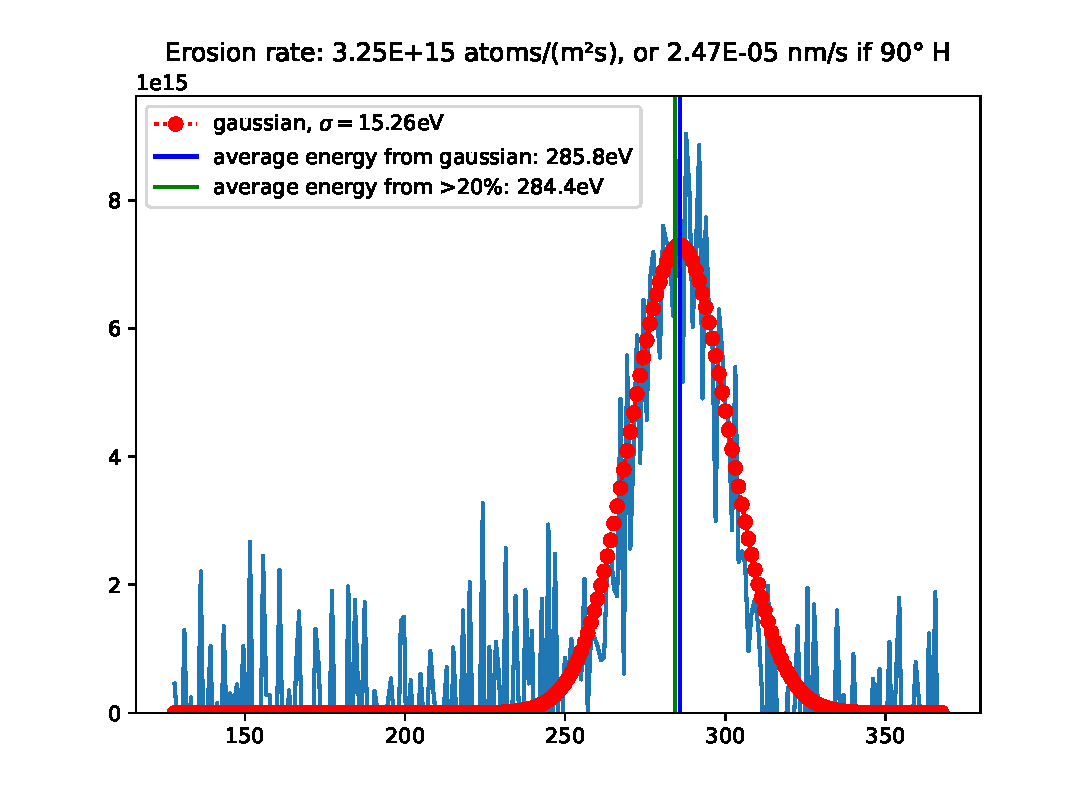
\includegraphics[width=\textwidth]{figures/ExampleIonDistribution.pdf}
\end{frame}
\begin{frame}
    \frametitle{sputtering depends on angle and projectile species}
    \includegraphics[width=0.8\textwidth]{figures/AngleDependance.pdf}\\
    We will assume worst case scenario: 80° and H2 majority plasma.
\end{frame}
\begin{frame}
    \frametitle{H2 100sccm GD current varience at 0mm}
    \begin{minipage}{0.49\textwidth}
        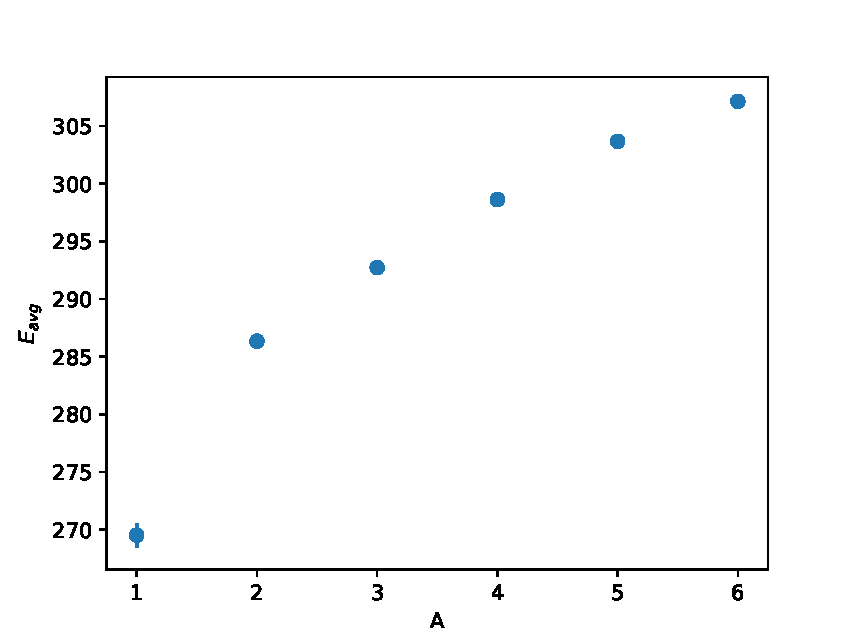
\includegraphics[width=1.1\textwidth]{figures/CurrentVary_H2_100sccm_Energy_werrors.pdf}
    \end{minipage}
    \begin{minipage}{0.49\textwidth}
        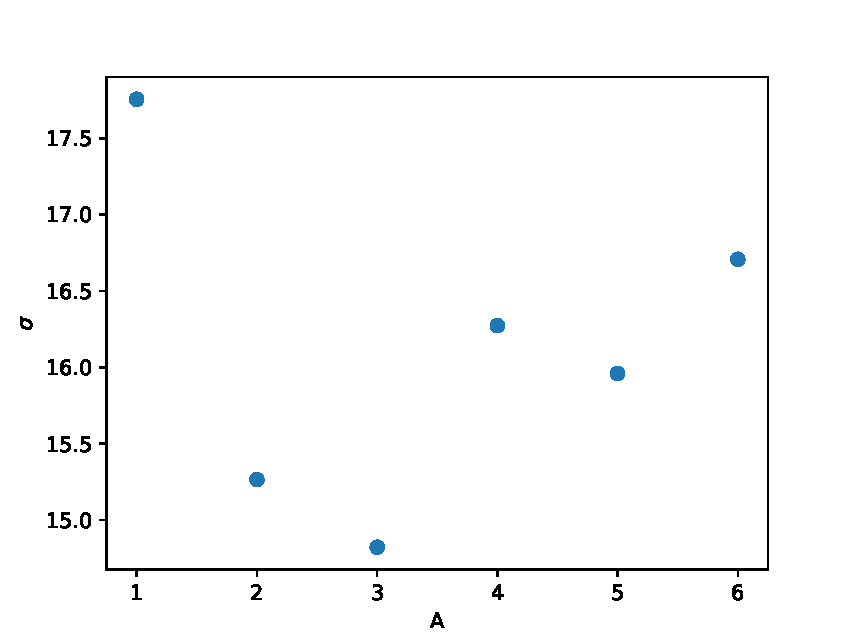
\includegraphics[width=1.1\textwidth]{figures/CurrentVary_H2_100sccm_Energy_sigma.pdf}
    \end{minipage}
    \begin{minipage}{0.49\textwidth}
        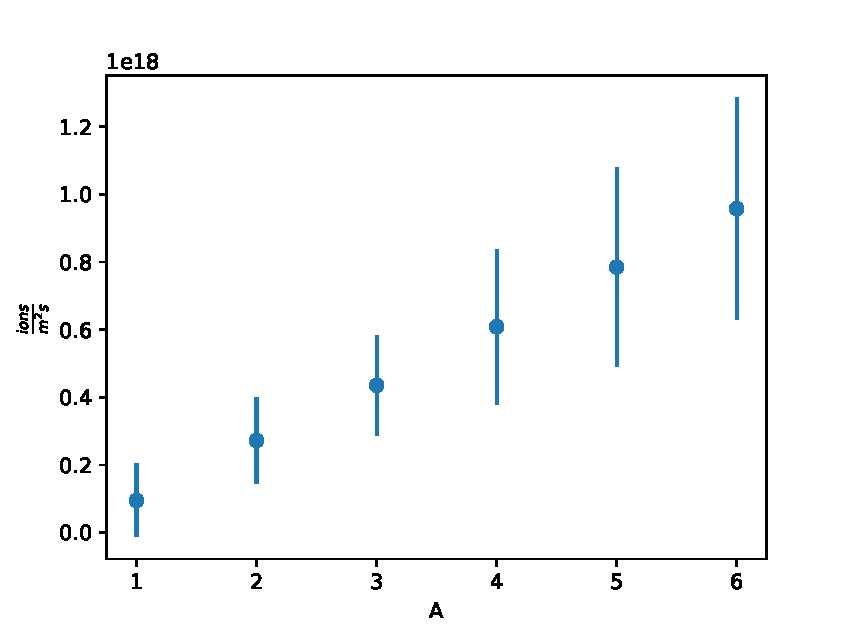
\includegraphics[width=1.1\textwidth]{figures/CurrentVary_H2_100sccm_flux_werrors.pdf}
    \end{minipage}
    \begin{minipage}{0.49\textwidth}
        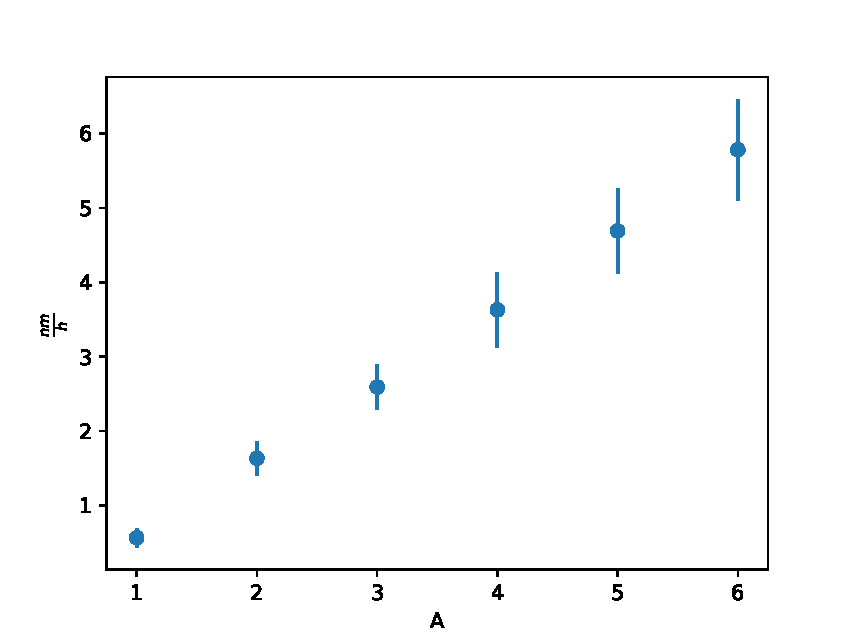
\includegraphics[width=1.1\textwidth]{figures/CurrentVary_H2_100sccm_worstcasesput_werrors.pdf}
    \end{minipage}
\end{frame}
\begin{frame}
    \frametitle{H2 2A gas amount varience at 0mm}
    \begin{minipage}{0.49\textwidth}
        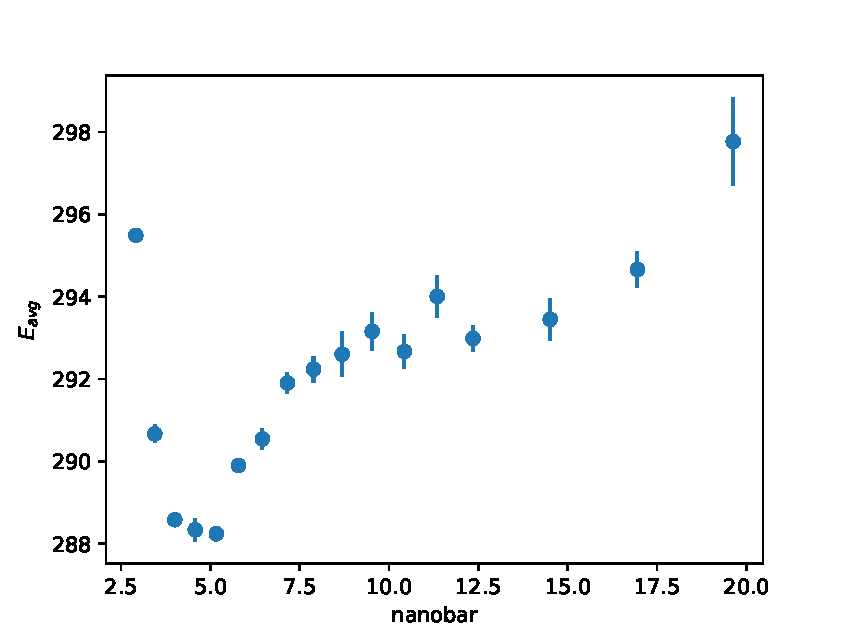
\includegraphics[width=1.1\textwidth]{figures/Gasvary_H2_2A_Energy_werrors.pdf}
    \end{minipage}
    \begin{minipage}{0.49\textwidth}
        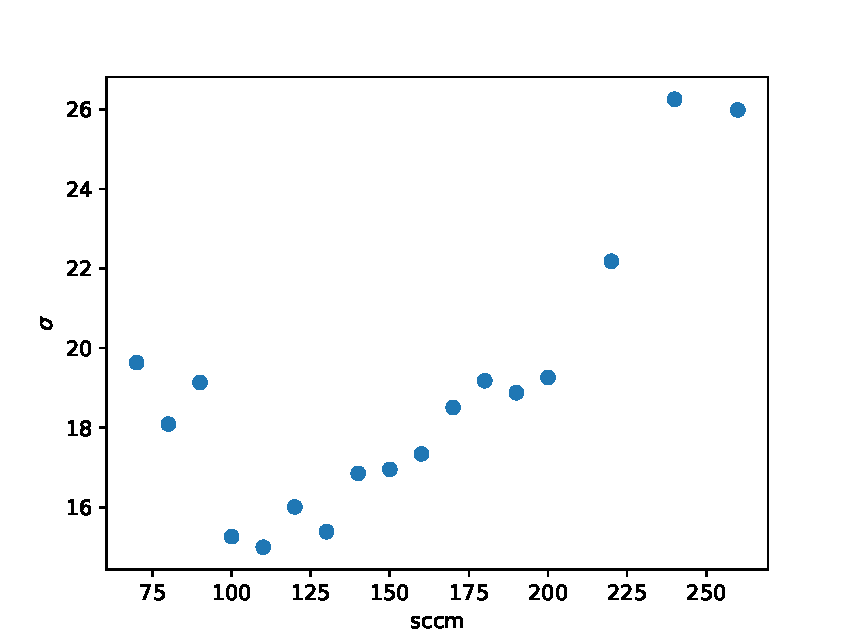
\includegraphics[width=1.1\textwidth]{figures/Gasvary_H2_2A_Energy_sigma.pdf}
    \end{minipage}
    \begin{minipage}{0.49\textwidth}
        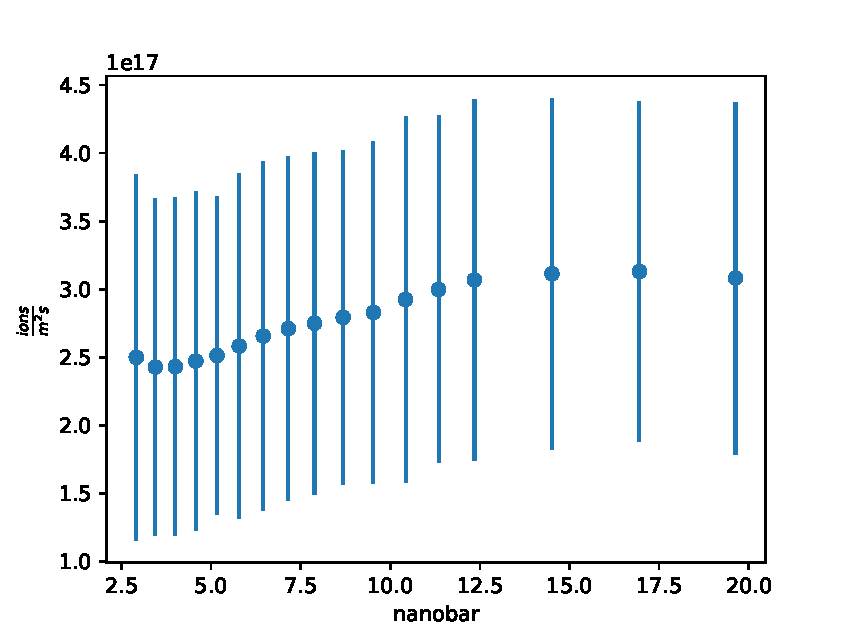
\includegraphics[width=1.1\textwidth]{figures/Gasvary_H2_2A_flux_werrors.pdf}
    \end{minipage}
    \begin{minipage}{0.49\textwidth}
        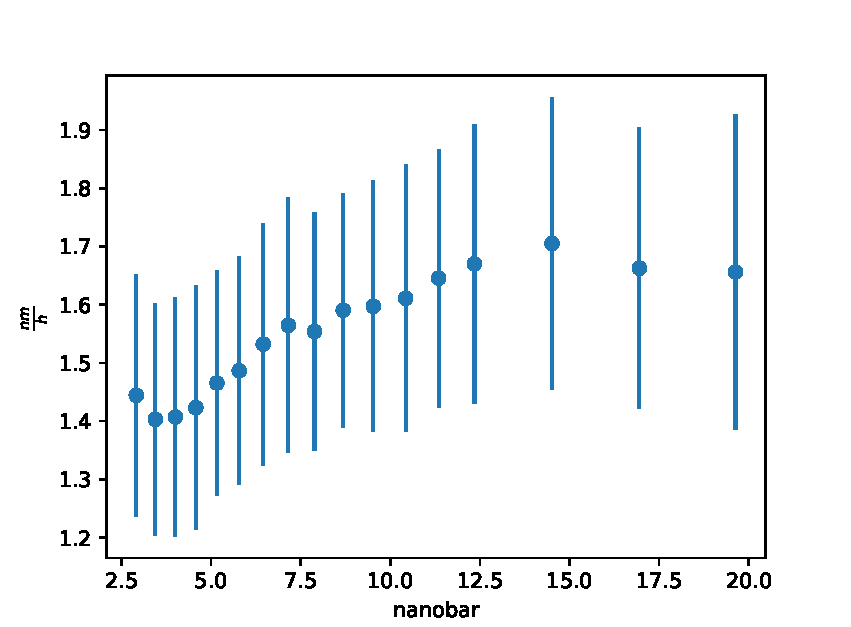
\includegraphics[width=1.1\textwidth]{figures/Gasvary_H2_2A_worstcasesput_werrors.pdf}
    \end{minipage}
\end{frame}
\begin{frame}
    \frametitle{H2 2A position varience at 100sccm}
    \begin{minipage}{0.49\textwidth}
        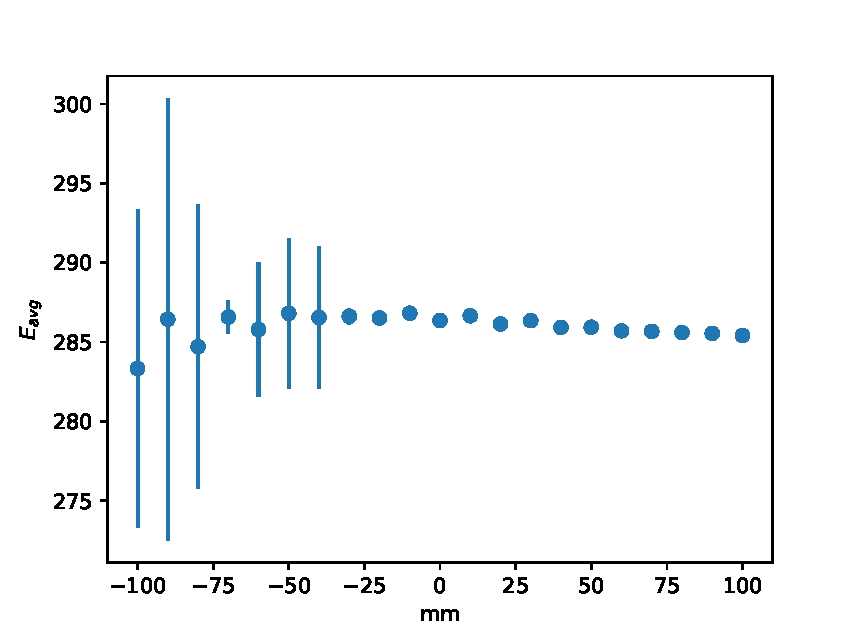
\includegraphics[width=1.1\textwidth]{figures/PosVary_H2_2A_Energy_werrors.pdf}
    \end{minipage}
    \begin{minipage}{0.49\textwidth}
        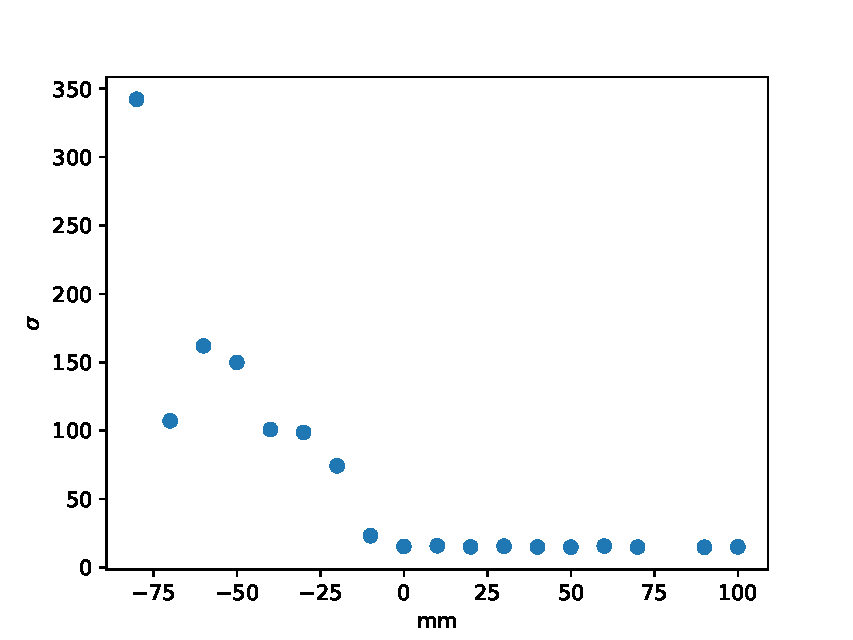
\includegraphics[width=1.1\textwidth]{figures/PosVary_H2_2A_Energy_sigma.pdf}
    \end{minipage}
    \begin{minipage}{0.49\textwidth}
        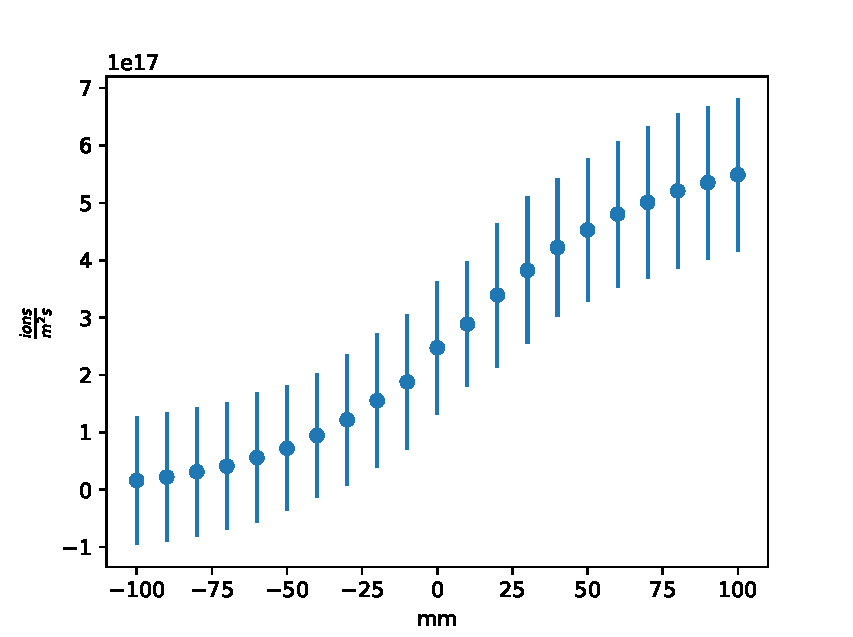
\includegraphics[width=1.1\textwidth]{figures/PosVary_H2_2A_flux_werrors.pdf}
    \end{minipage}
    \begin{minipage}{0.49\textwidth}
        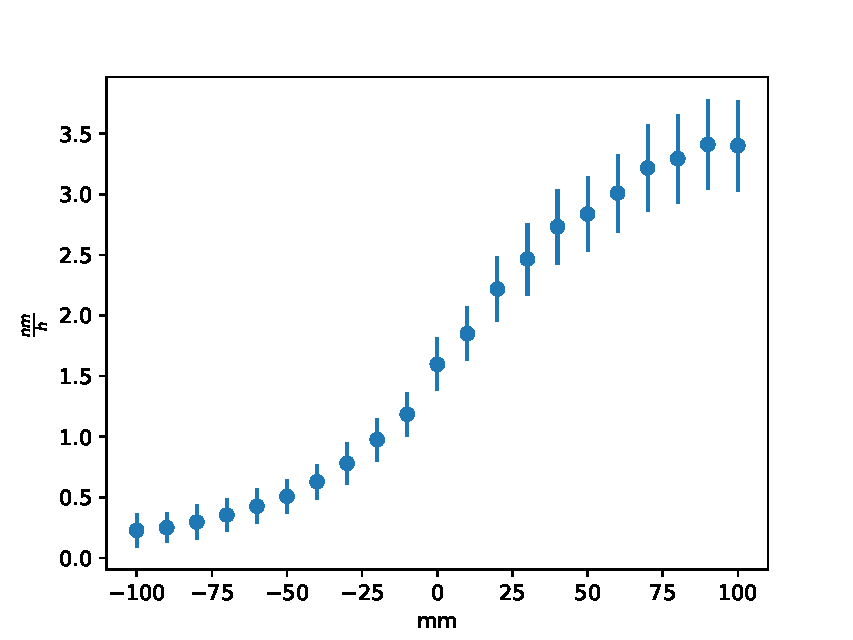
\includegraphics[width=1.1\textwidth]{figures/PosVary_H2_2A_worstcaseput_werrors.pdf}
    \end{minipage}
\end{frame}
\begin{frame}
    \frametitle{less conservative erosion estimates}
    \begin{minipage}{0.49\textwidth}
        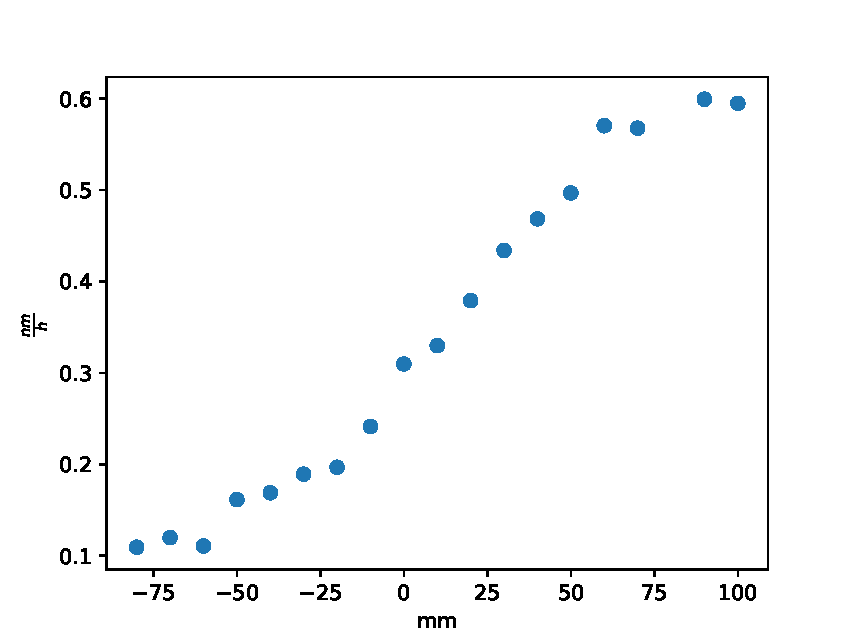
\includegraphics[width=1.1\textwidth]{figures/PosVary_H2_2A_sput.pdf}
    \end{minipage}
    \begin{minipage}{0.49\textwidth}
        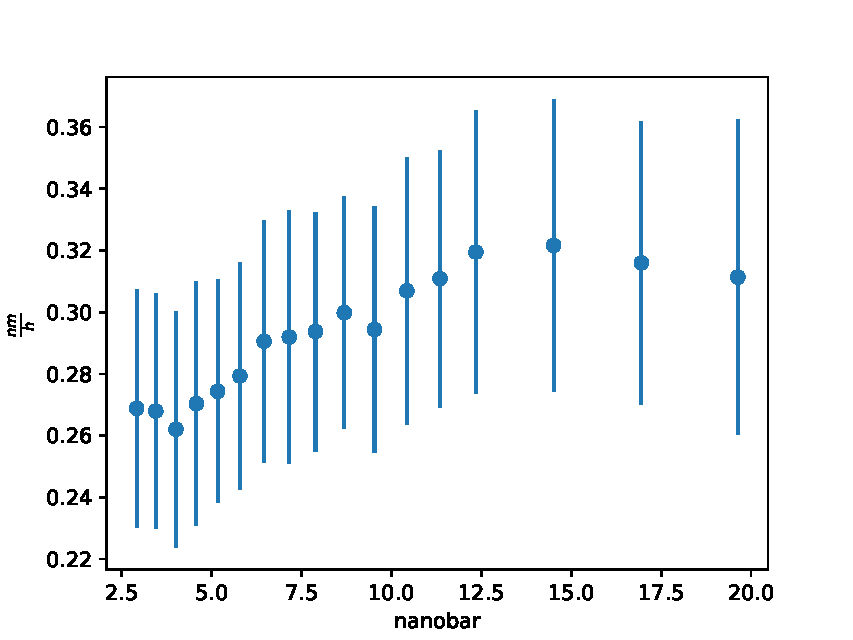
\includegraphics[width=1.1\textwidth]{figures/Gasvary_H2_2A_sput.pdf}
    \end{minipage}
    \begin{minipage}{0.49\textwidth}
        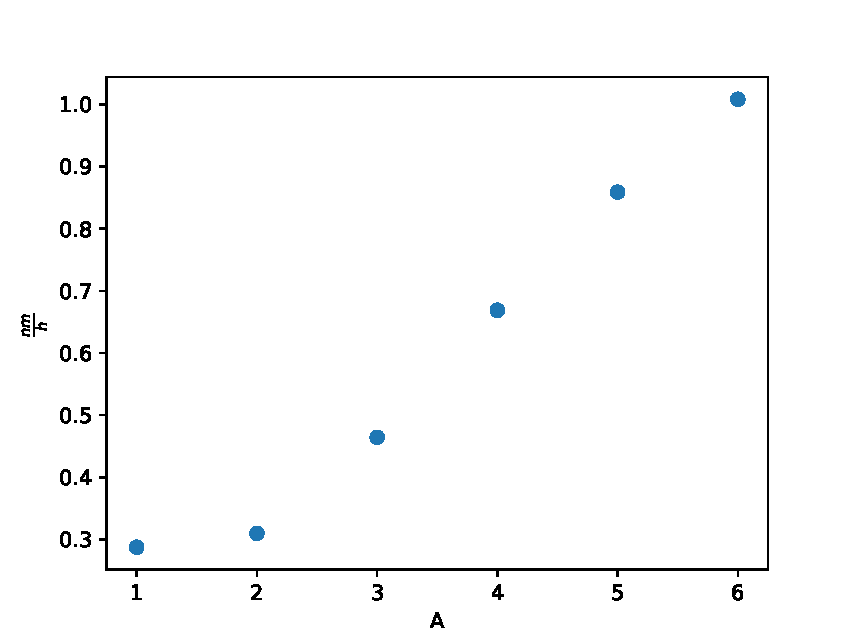
\includegraphics[width=1.1\textwidth]{figures/CurrentVary_H2_100sccm_sput.pdf}
    \end{minipage}
    \hspace{0.5cm}
    \begin{minipage}{0.39\textwidth}
        Hydrogen ions
        equally likely angle distribution
    \end{minipage}
\end{frame}
\end{document}

